

    (Fill in bits about the squeezer)

    \section{Squeezing theory}
    \label{squeezing_theory}

        Squeezing theory.

        \subsection{Quantum shot noise and radiation pressure}
        \label{quantum_noise}

            Carlton Caves, quantum shot noise and radiation pressure.

        \subsection{Problems with lasers: thermal compensation}
        \label{TCS}

            Experience (some firsthand) with thermal compensation.

        \subsection{Squeezing filter cavities against alternatives}
        \label{third-gen_squeezing}

    \section{LIGO Hanford Observatory quantum vacuum squeezing}
    \label{LHO_squeeze}

        Quantum vacuum squeezing at LIGO Hanford Observatory. Naturally, a great deal of description and background will come from Sheila Dwyer's thesis~\cite{DwyerThesis} and Sheon Chua's thesis~\cite{ChuaThesis}.

        \subsection{Collaboration and contributions}
        \label{contributions}

            Contributions: table, in-vacuum installation, electronics, range est.

            \subsubsection{Optical table support assembly}
            \label{table_legs}

                Table legs (me) and results of Sheon and Robert's shakers.

		Here might be good place to put old AutoCAD drawings to use.

            \subsubsection{Faraday isolator measurement}
            \label{Faraday}

                Faraday isolator measurement (me with Keita, Matt, Lisa).

		What were the results of the measurement? Show e-log entries, comment on in-and-out-of-vacuum performance and what it says about the need for low loss to be a top priority in future squeezing efforts.

            \subsubsection{In-vacuum installation}
            \label{In-vacuum}

                In-vacuum Faraday and baffle installation with "".

                Show pictures of the installation, connect to the issues with stray and perhaps backscattered light.

		Discuss the repair of the output mode cleaner, which is mentioned (citation 50) in Nic's thesis~\cite{SmithThesis}. The technical report corresponding to it is by Waldman and Chua~\cite{Waldman2011}.

            \subsubsection{Data digitization}
            \label{data_digitization}

                Electronic cabling and analog-to-digital converter installation.

		May want helpful diagram.

            \subsubsection{Figures of merit: inspiral range}
            \label{range_est}

                Range estimation after squeezing

		From the improved shot noise, we can see that squeezing at high frequencies bought enhanced LIGO a megaparsec of inspiral range. This number is impressive in several respects: our goal was to acheive a squeezing factor of perhaps as much as 3 dB, but to do it in the shot noise-limited region, at high frequencies, where the inspiral range equations (MATH: add the inspiral range equation if not already shown for feedforward!) count for much less. Morever, that range figure reflects the acheivement of squeezing down to 150 Hz (CITE: can we use this number?), which is the lowest yet achieved for a gravitational wave interferometer.

        \subsection{Success and Advanced LIGO prospects}
        \label{squeezing_success}

            Results and hopes for aLIGO+ squeezing.

	    The squeezer group has a paper pending in review for Nature, written by Lisa Barsotti, in which we discuss our acheivement of perhaps 2 dB worth of squeezing (need to cite and check whether it is OK to use this number)~\cite{BarsottiNatureSqueezing}. It builds on the previous success of GEO600 in squeezing~\cite{GEO600NatureSqueezing}.

	    Discuss Sheila Dwyer's~\cite{DwyerPhaseNoise} and Sheon Chua's~\cite{ChuaBackscatteredLight} papers, since I am an author on both of them. We have a preliminary understanding now of at least two major problems: the quadrature phase noise fluctatuations and backscattered light. Backscattered light can be resolved in several ways. Phase noise must be progressively improved, as Sheila discusses, because we can hope to acheive the mature filter cavity design proposed below.

Discuss Lisa Barsotti's talk about the future prospect for LIGO using filter cavities, work that Tomoki Isogai is doing. With filter cavities, we can acheive frequency-dependent squeezing, having the best of both works by reducing quantum radiation pressure noise at low frequencies and shot noise at high, by using the filter cavity to produce a squeezed vacuum with a squeeze angle that varies as a function of frequency. Though as yet this filter cavity has yet to be constructed, it is in the works at MIT.

% Everything below is imported from my AEI talk

\section{Squeezing large interferometers}
%\begin{frame}{Squeezing introduction}

%\begin{definition}
Altering $\Delta E\Delta\phi$ uncertainty for the electromagnetic
field
%\end{definition}
\begin{itemize}
\item Demonstrated first at GEO 600, then LIGO Hanford (H1)\end{itemize}
\begin{theorem}
Shot noise arises from quantum operators (Caves 1980, 1981)\end{theorem}
\begin{itemize}
\item Vacuum fluctuations couple through anti-symmetric port
\item \emph{Squeeze }the $\overrightarrow{E}$ field uncertainty ellipse
\item Angle $\theta$, factor $r$, creation operator $a$, squeeze operator
$S$:
\end{itemize}

\[
S(\zeta)=\exp[\frac{1}{2}\zeta^{*}a^{2}-\frac{1}{2}\zeta(a^{\dagger})^{2}],\;\zeta=re^{i\theta}
\]



Squeezed state made with


optical parameter oscillator, 2nd harmonic generator


\textbf{Shot noise reduced by $e^{-r}$}


\[
\]


%\end{frame}

%\begin{frame}{Squeezing large interferometers}


\begin{figure}
%\protect\caption{\protect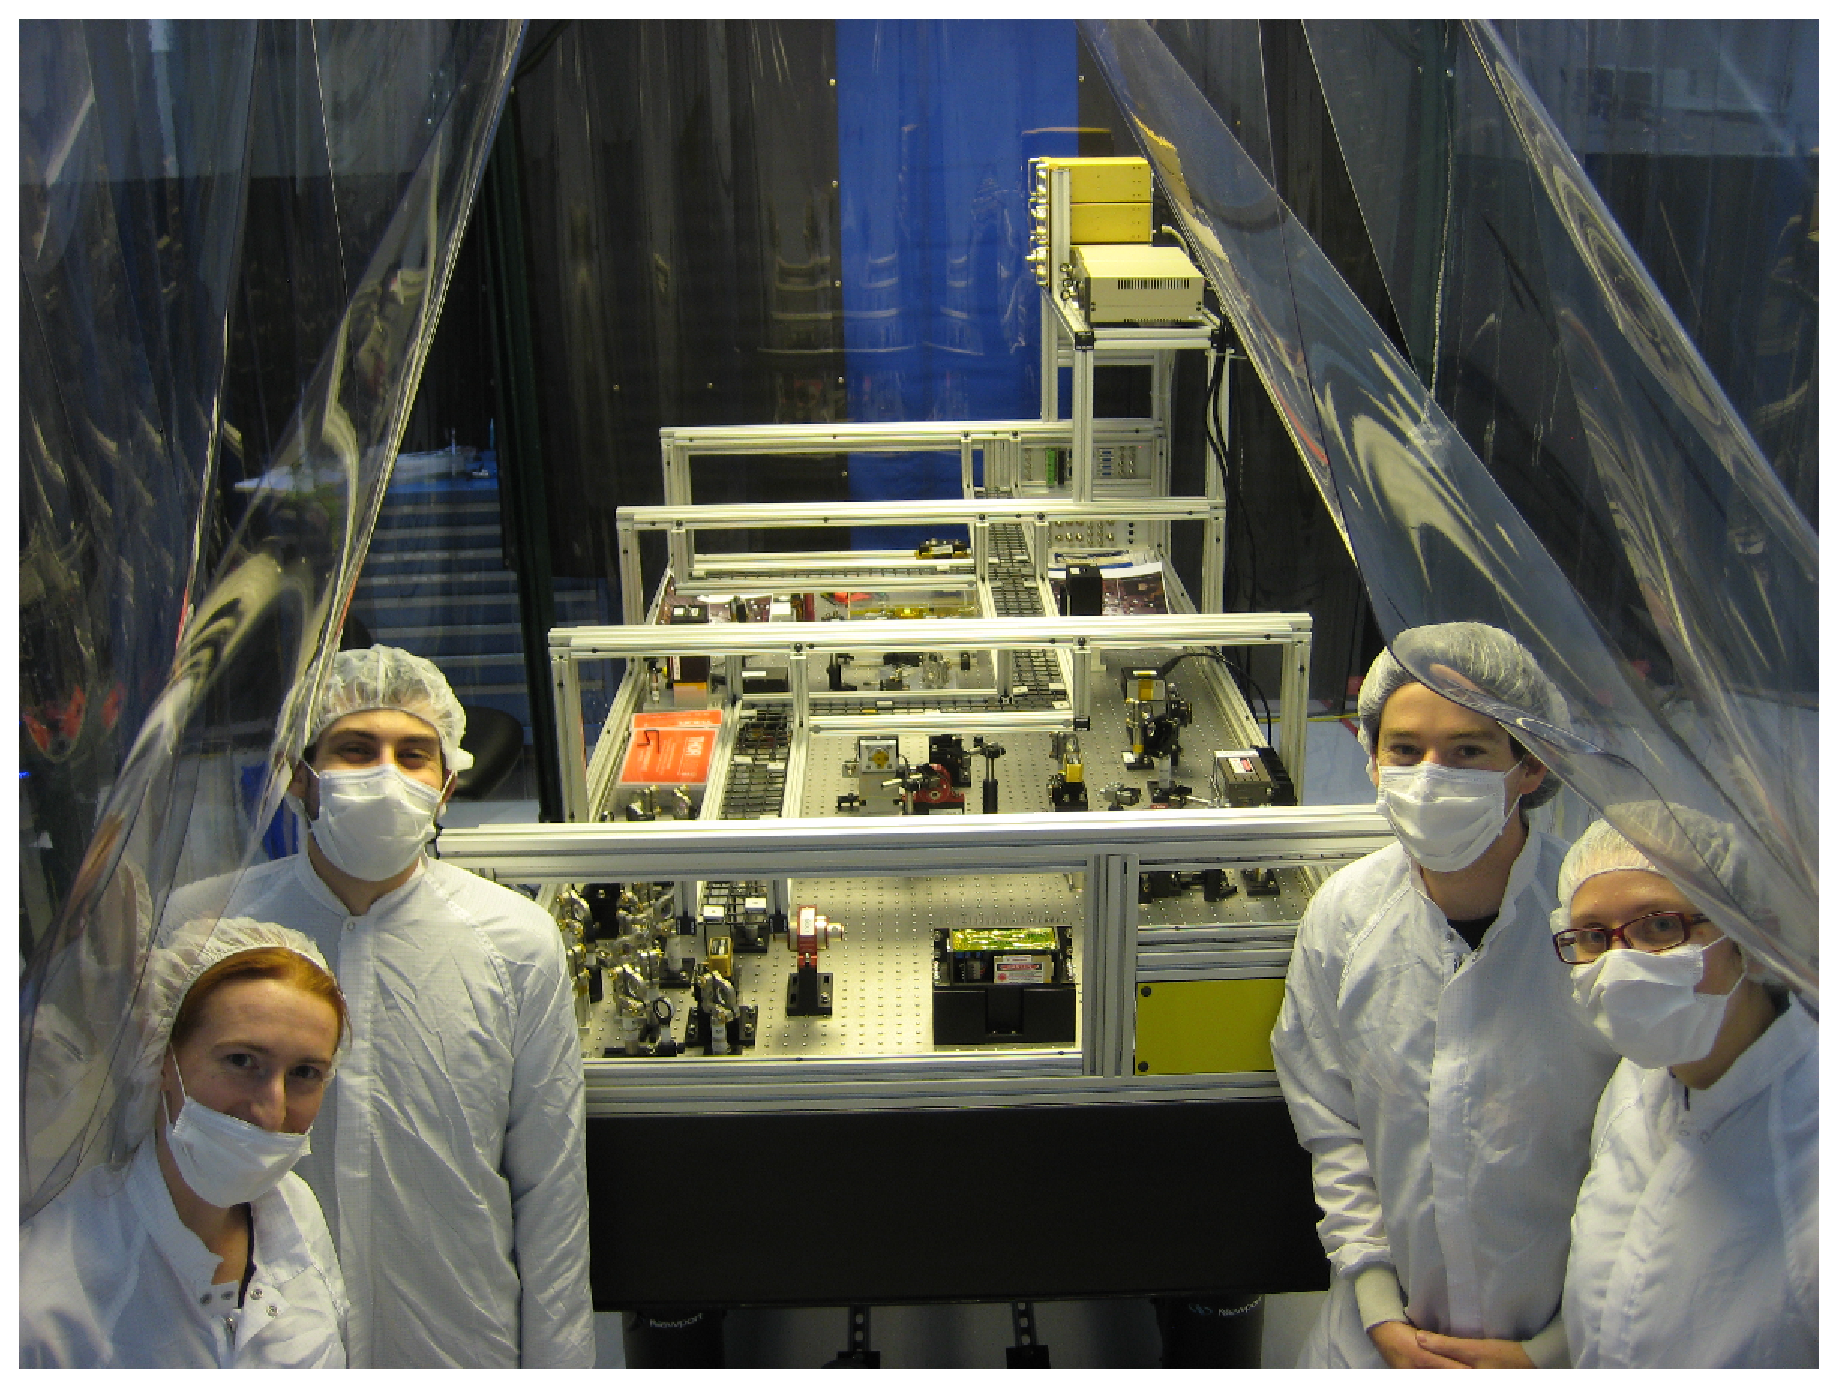
\includegraphics[width=0.33\paperwidth]{lisabar-1289966130}}
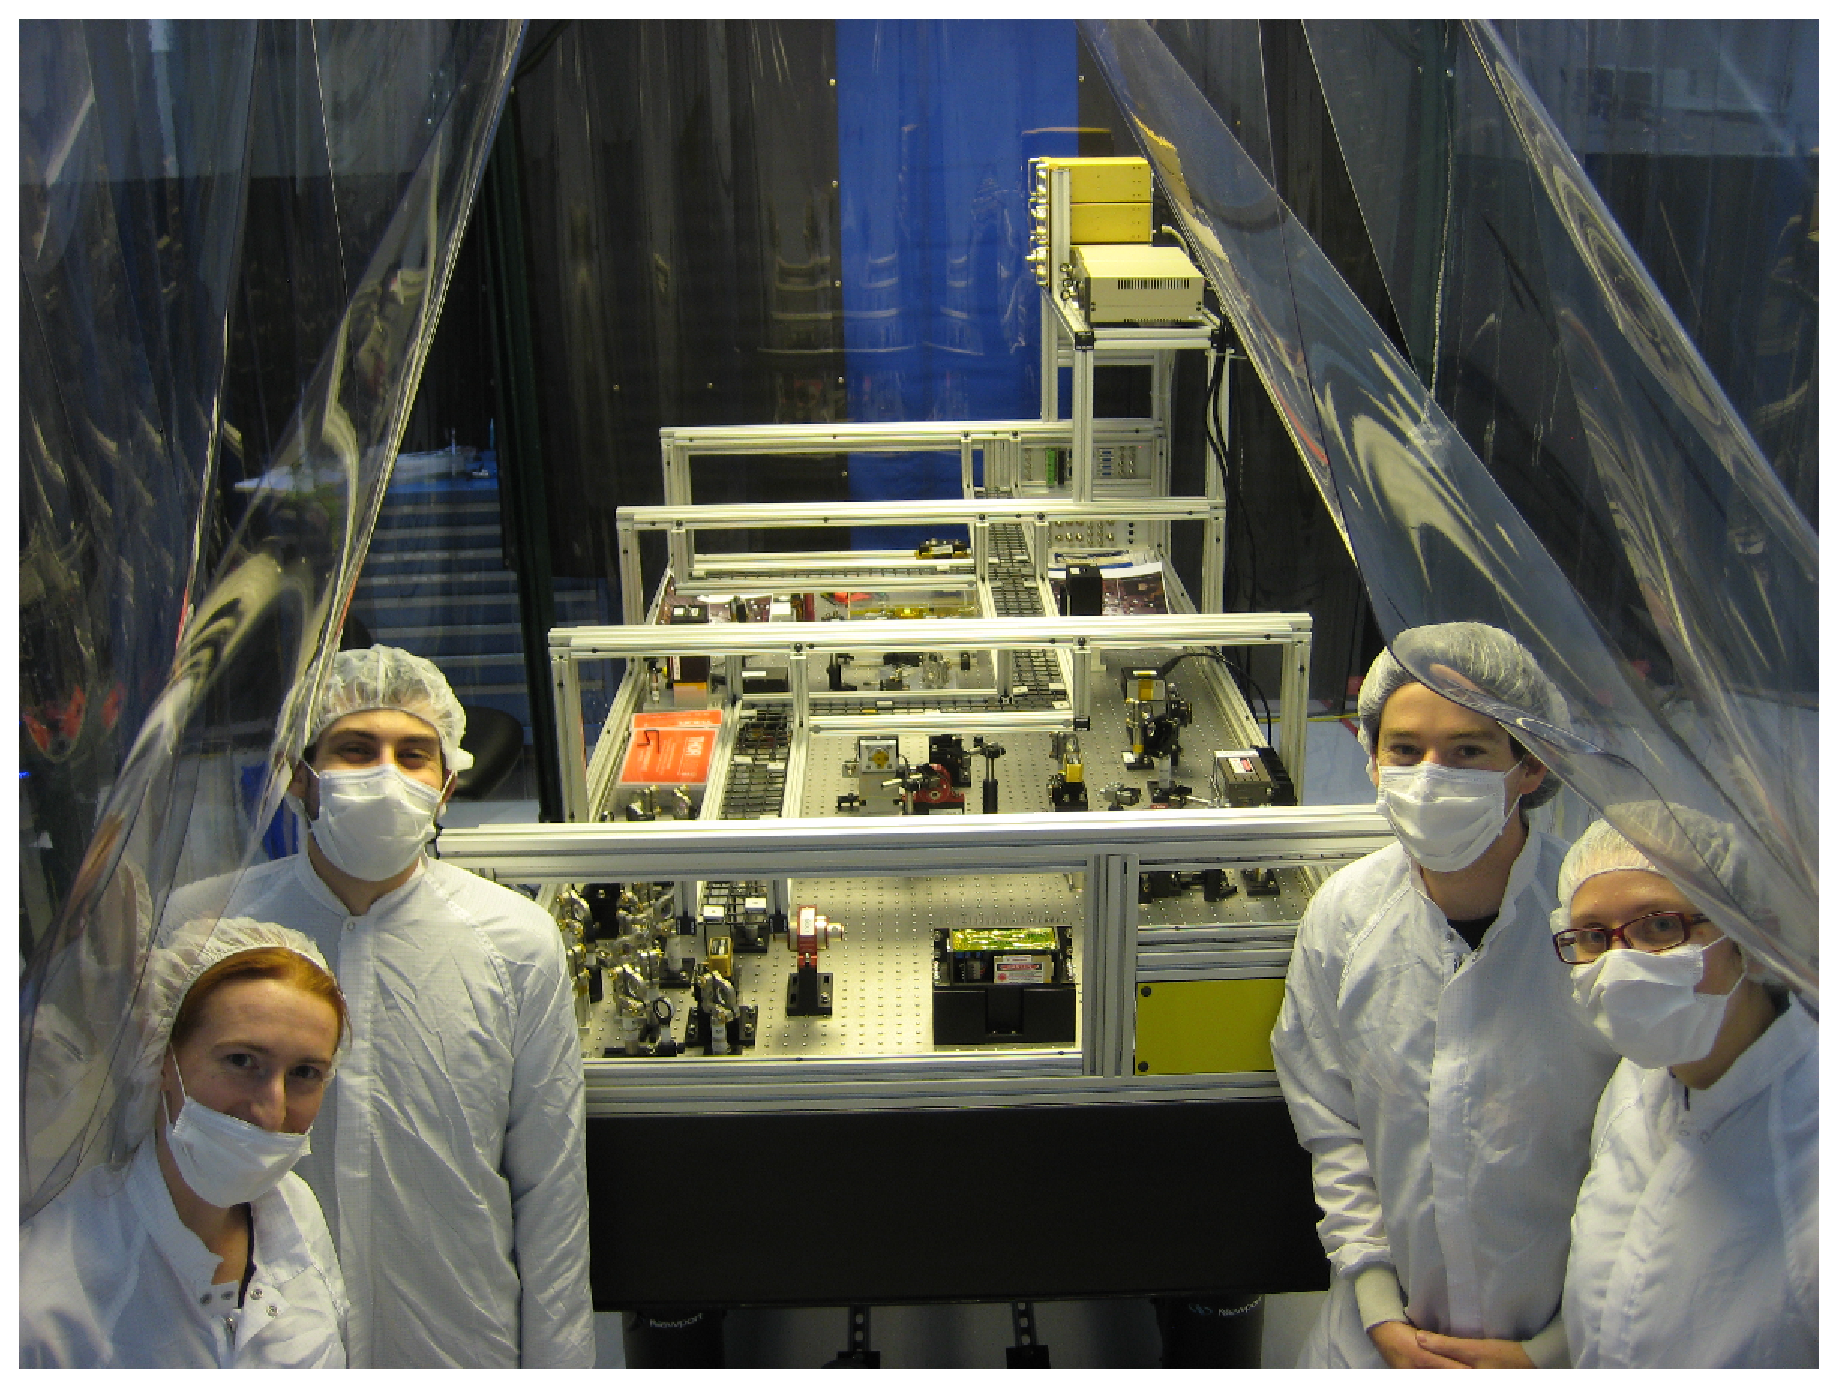
\includegraphics[width=0.6\paperwidth]{lisabar-1289966130.eps}


%\protect\caption{\protect\includegraphics[width=0.33\paperwidth]{lisabar-1300943141}}


\caption{Image by Lisa Barsotti in Hanford eLog
\newline CC from LL, Dwyer, Barsotti, Mow-Lowry, Meadors
}
\end{figure}
\begin{figure}
\includegraphics[width=0.6\paperwidth]{lisabar-1300943141.eps}
\caption{Table legs (\& helped w/ Faraday isolator, data channels)
}
\end{figure}


%\end{frame}

%\begin{frame}{Squeezing's scientific benefit}
\subsection{Squeezing's scientific benefit}


\begin{figure}
%\protect\caption{\protect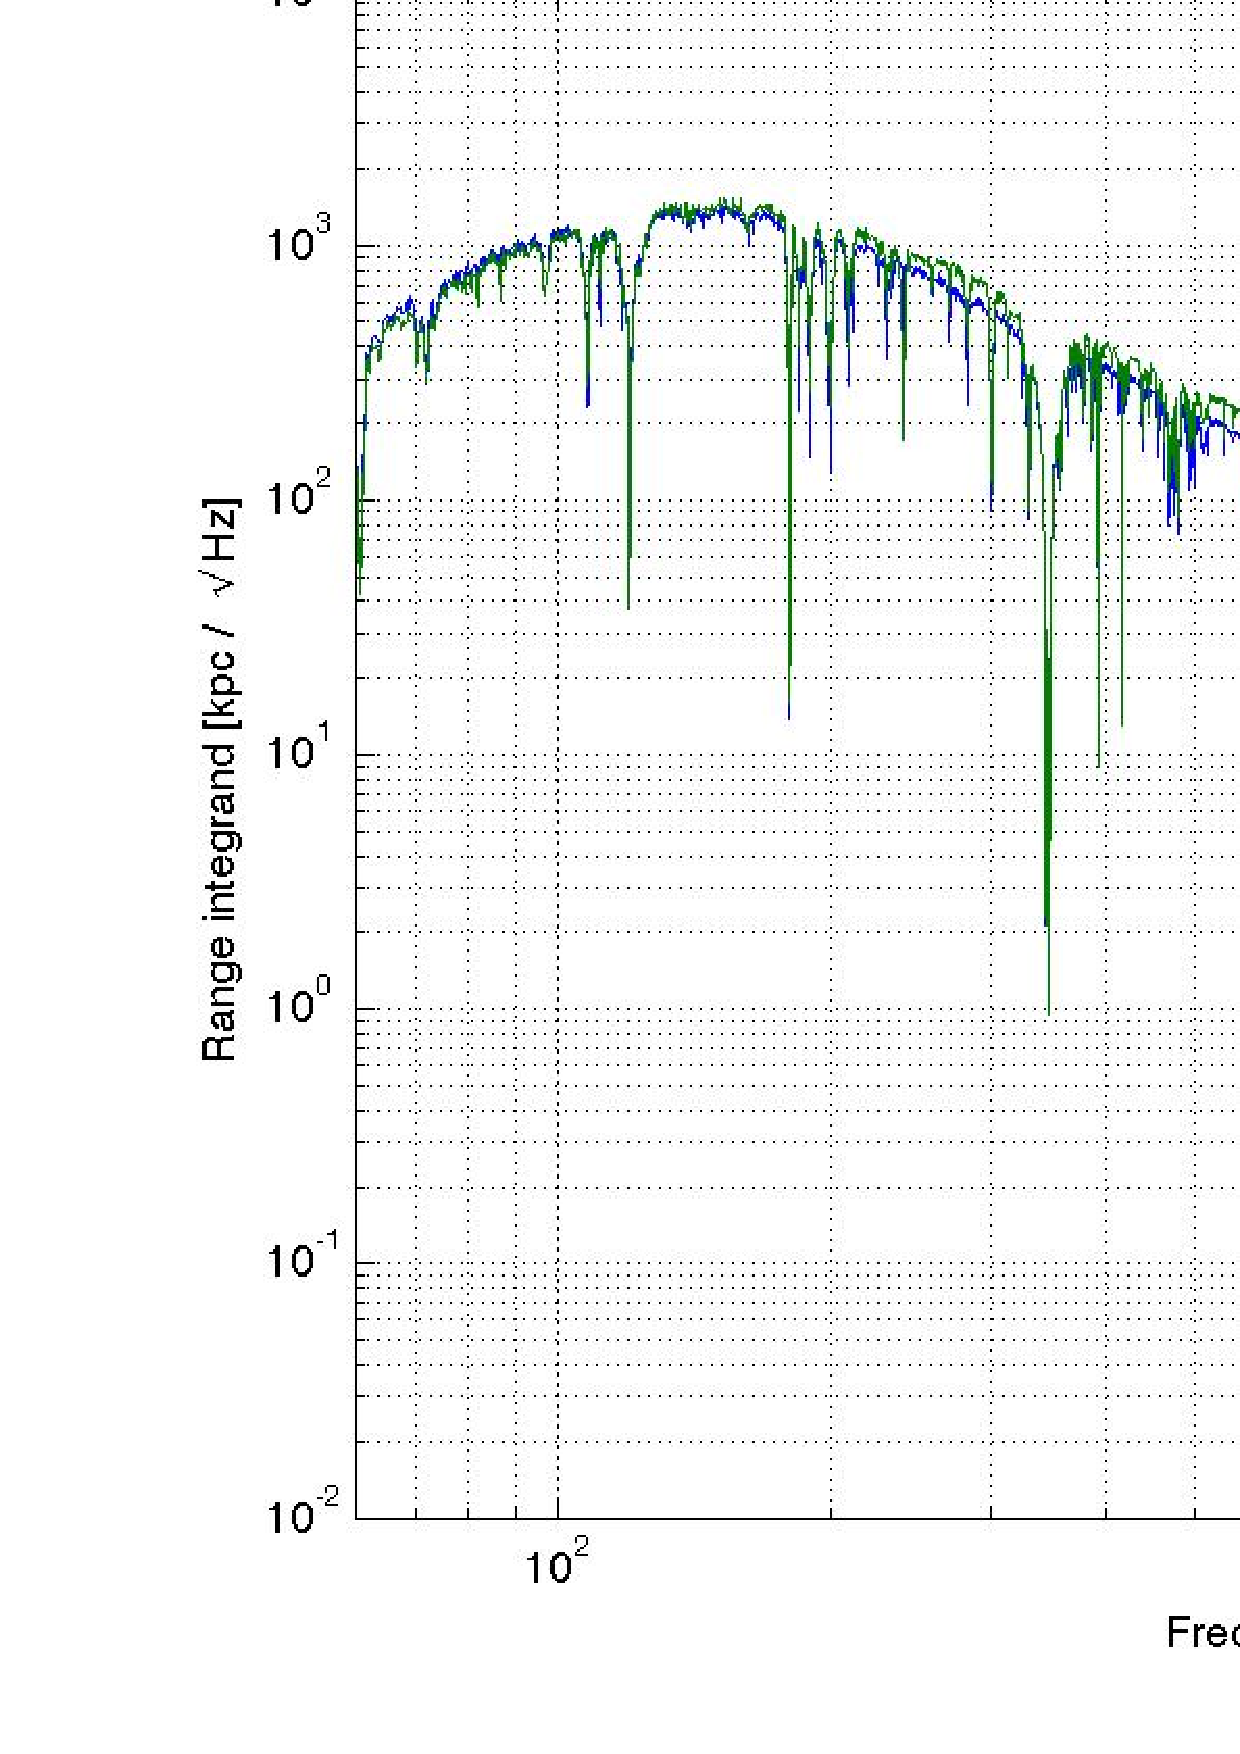
\includegraphics[width=0.45\paperwidth,height=0.45\paperheight,keepaspectratio]{range_integrand.jpeg}\protect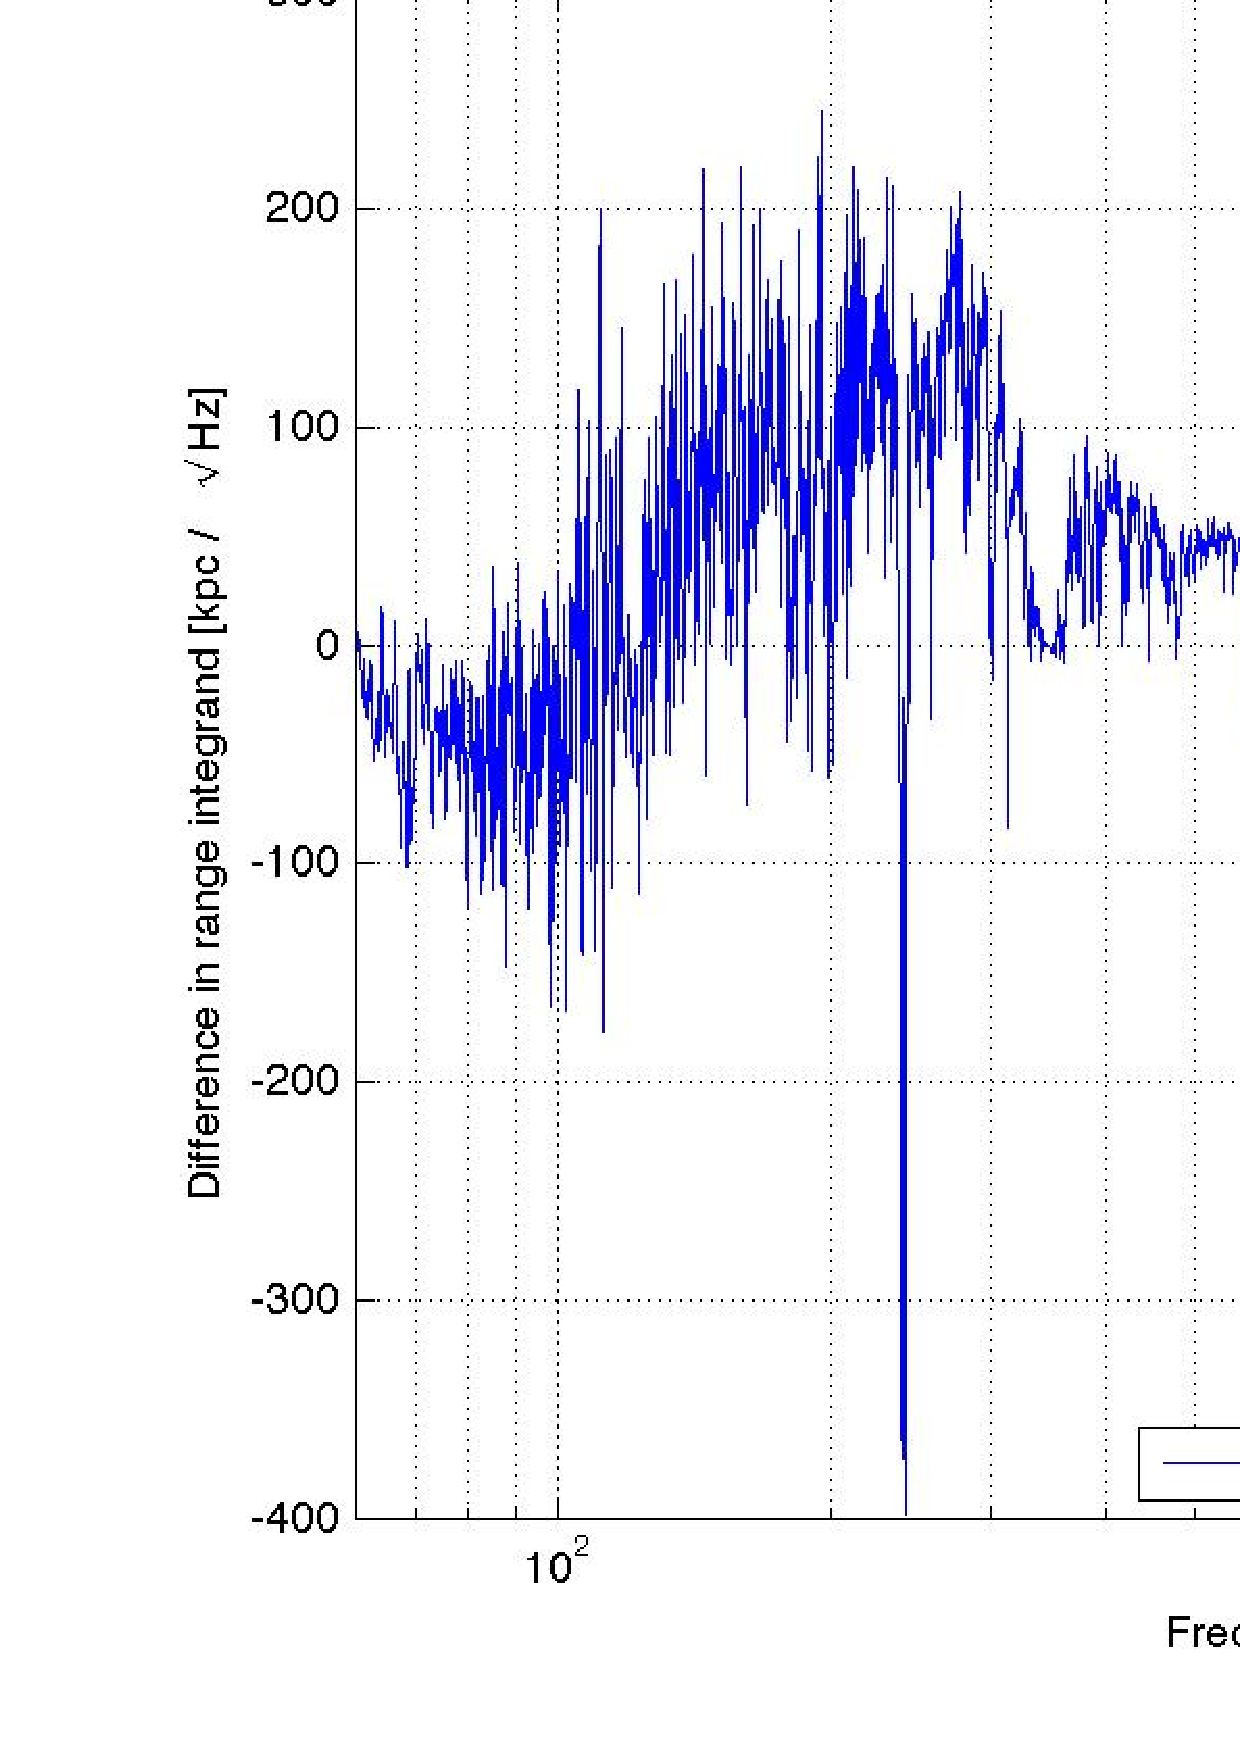
\includegraphics[width=0.45\paperwidth,height=0.45\paperheight,keepaspectratio]{range_integrand_difference.jpeg}}
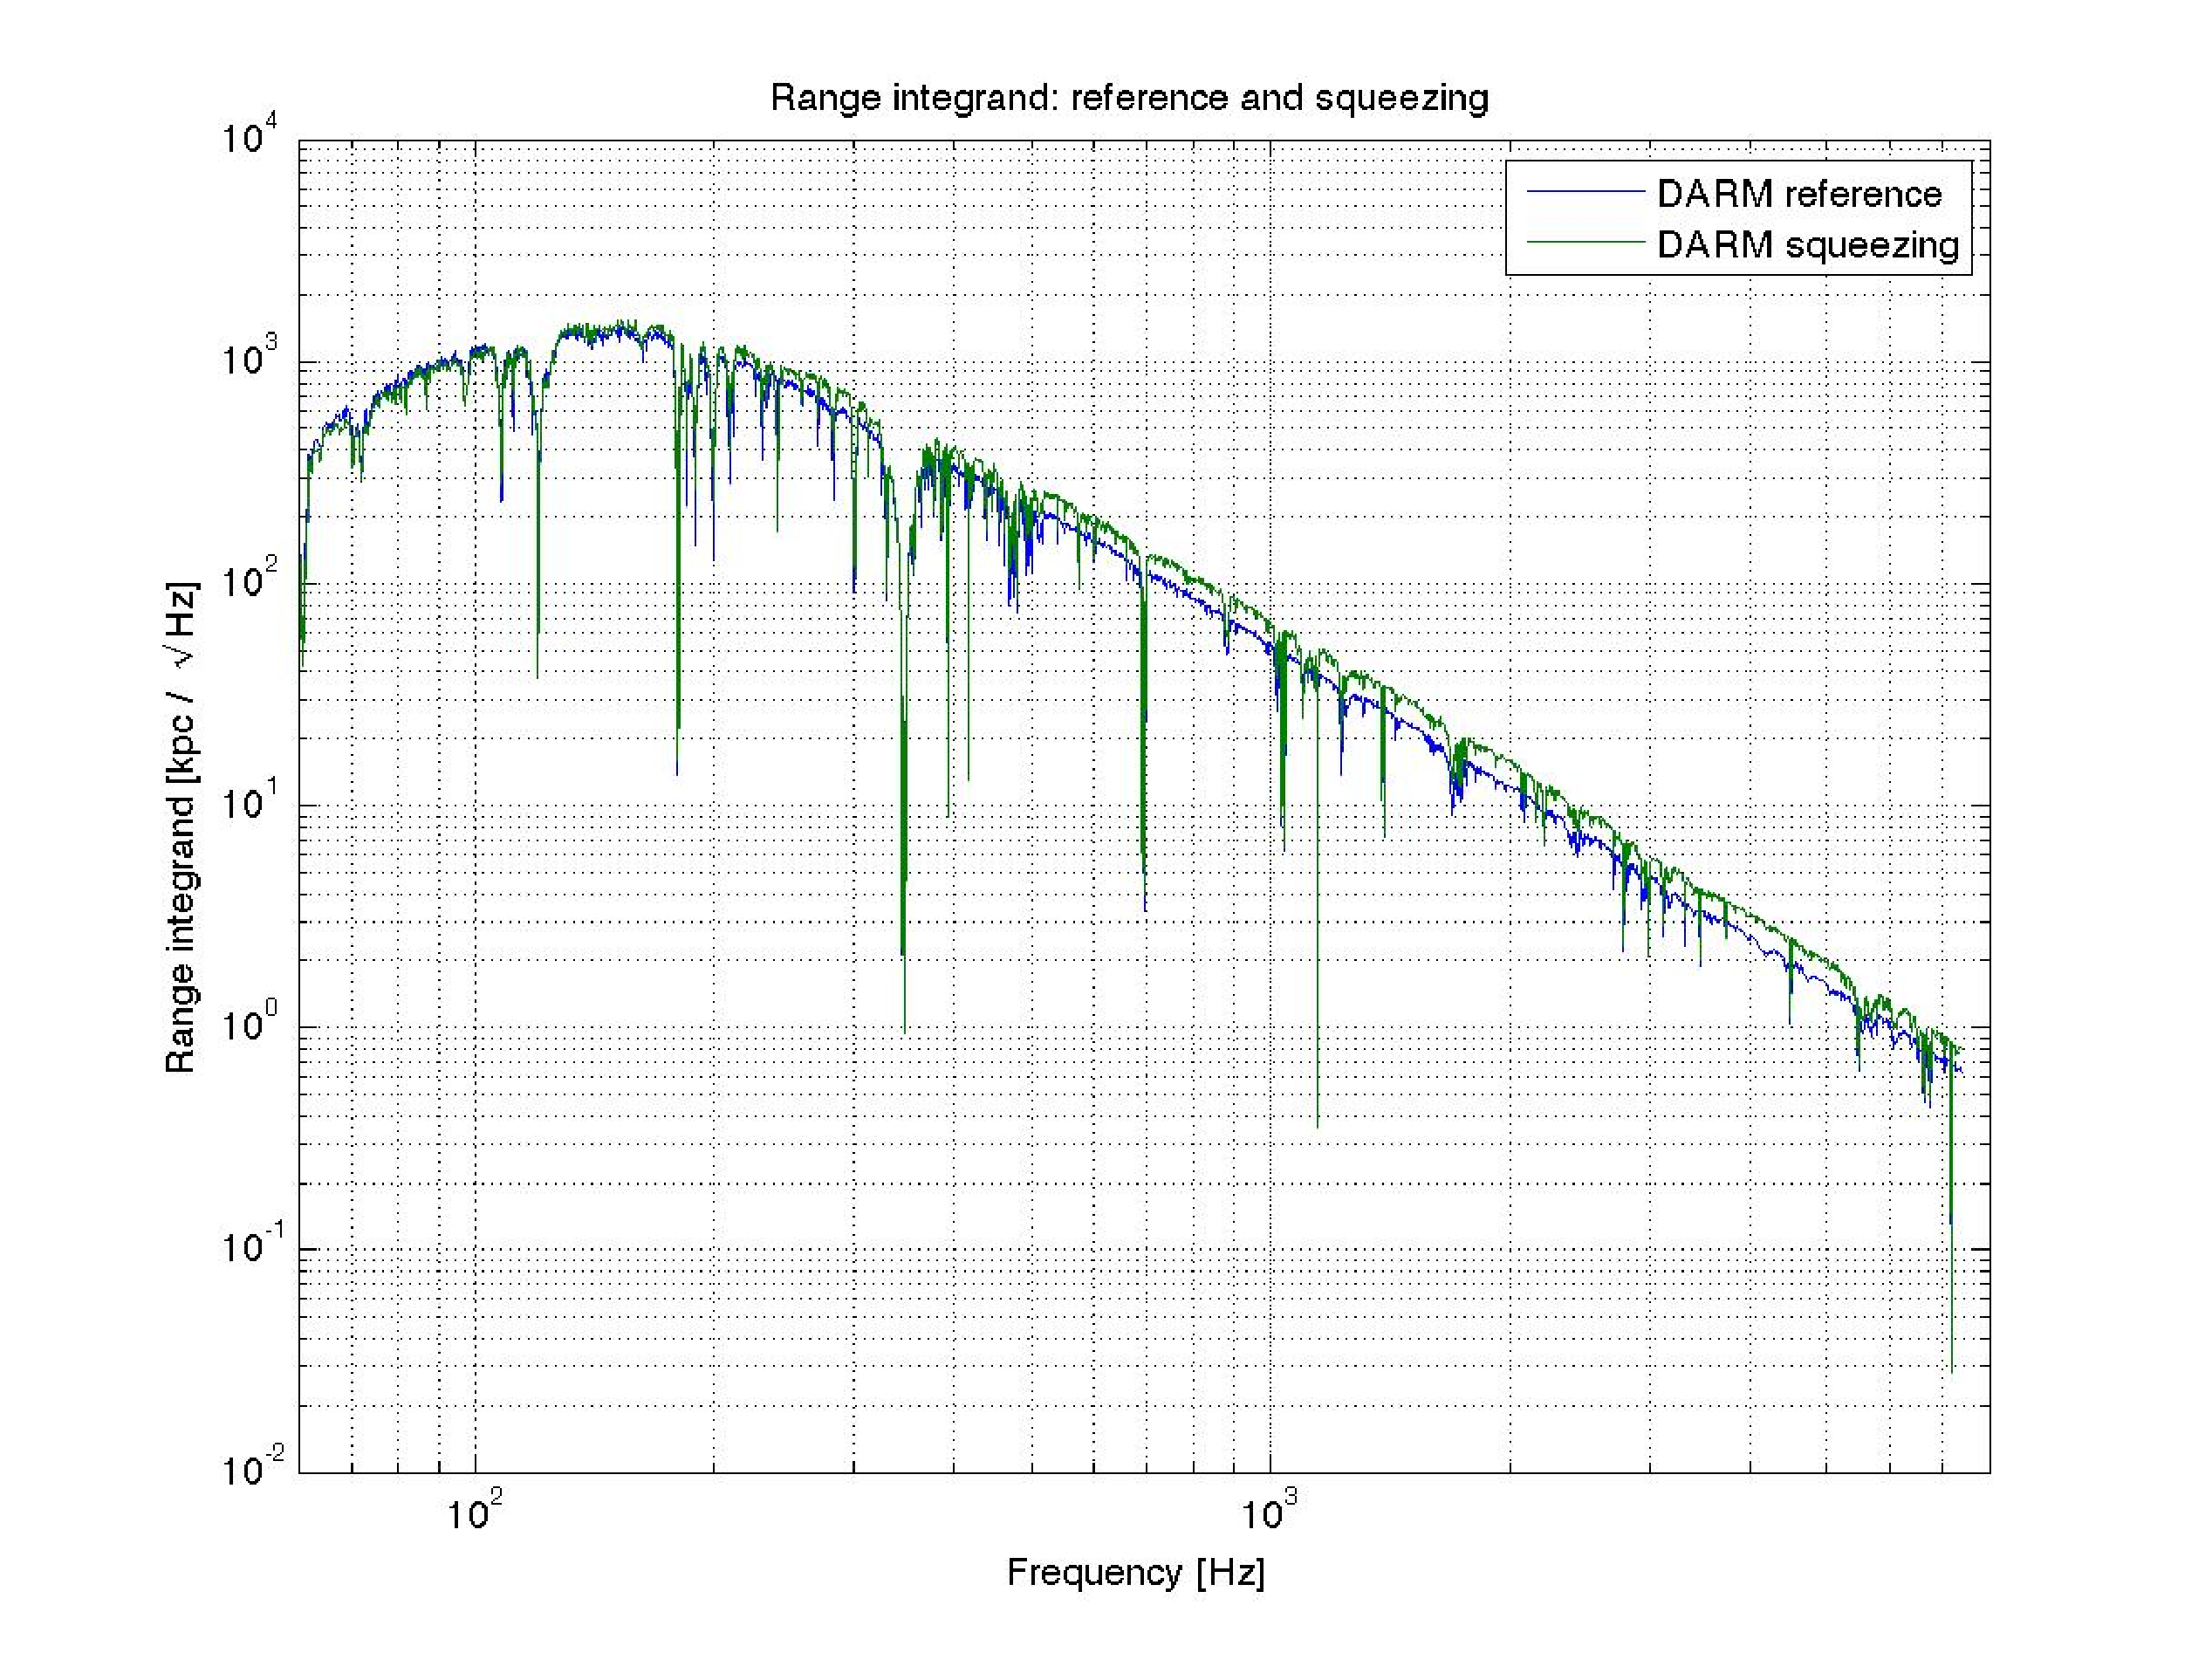
\includegraphics[height=0.5\paperheight, width=0.5\paperwidth,keepaspectratio]{range_integrand.eps}
\caption{Integrand of inspiral range as a function of frequency}
\end{figure}
\begin{figure}
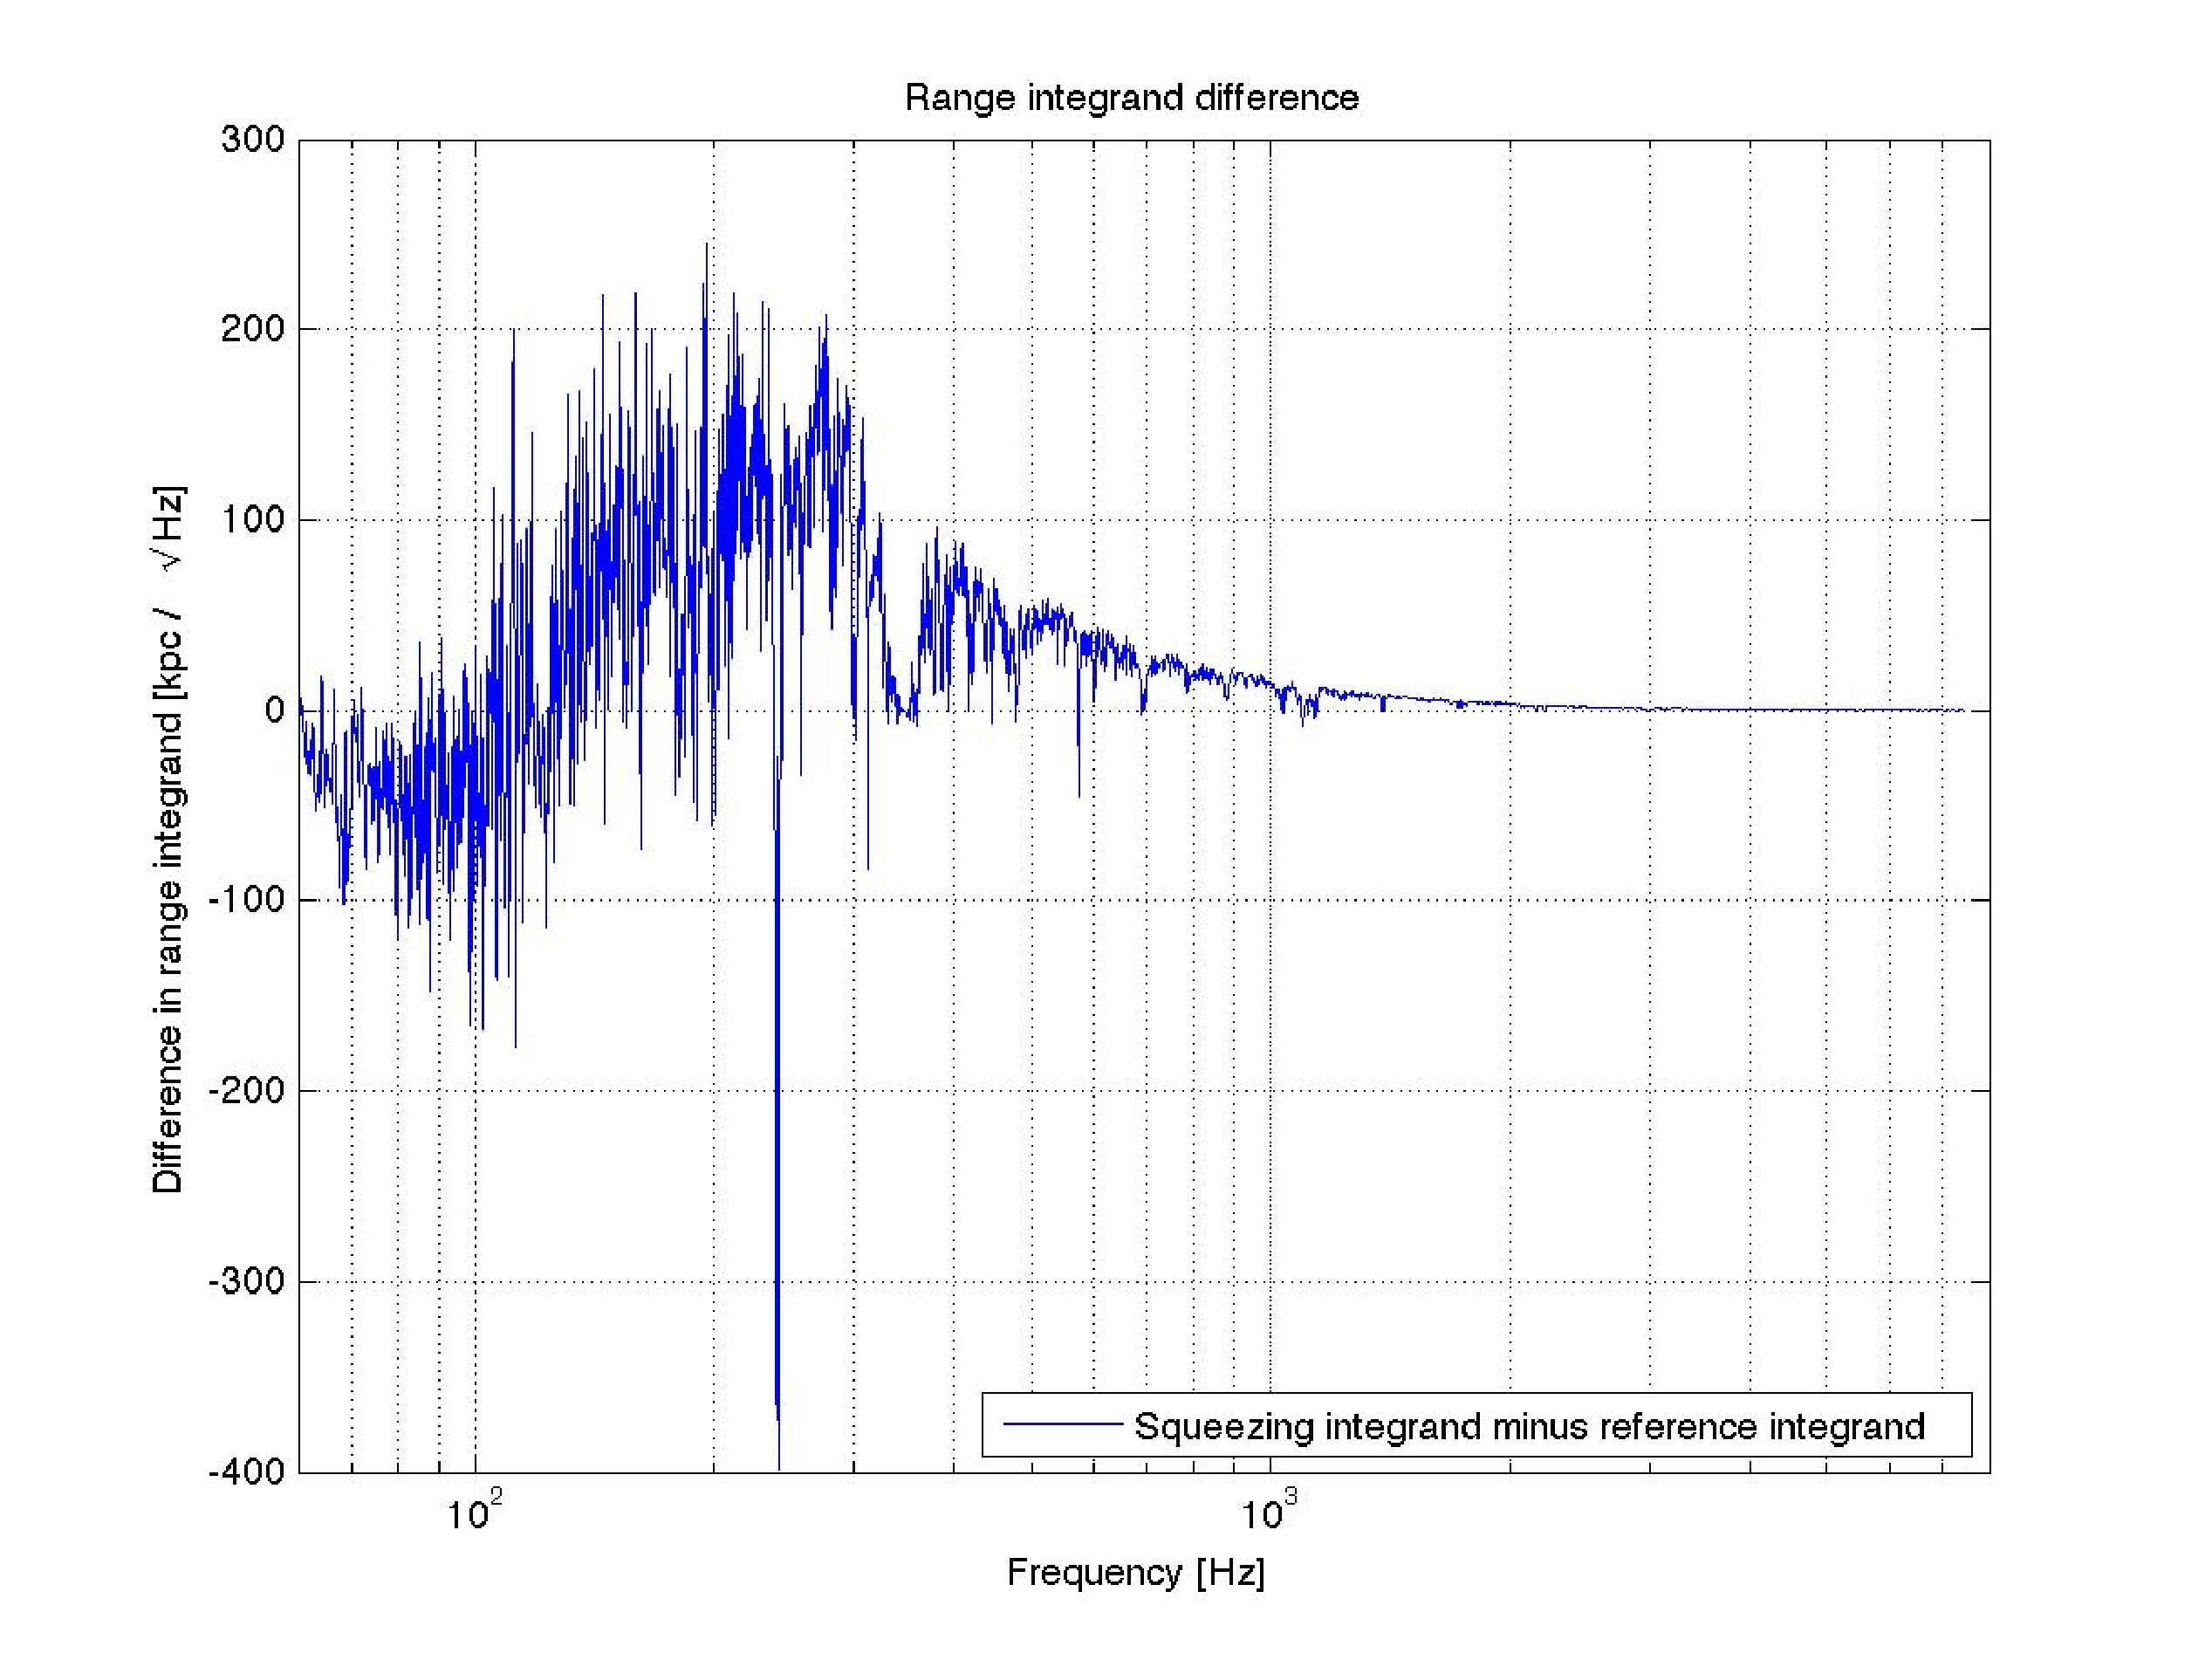
\includegraphics[height=0.5\paperheight, width=0.5\paperwidth,keepaspectratio]{range_integrand_difference.eps}
\caption{Net effect of squeezing on inspiral range integrand
\newline Scientific benefit at few hundred Hz $\rightarrow$ all ways to improve are good
}
\end{figure}


%\end{frame}

%\begin{frame}{Squeezing summary}
\subsection{Squeezing summary}

\begin{description}
\item [{Instrumental}] experience with technique important beyond Advanced
LIGO
\item [{Physical}] way to improve broad band of LIGO, benefit many searches
\item [{Illustrates}] need for best sensitivity at few hundred Hz
\item [{Question}] what can we improve \emph{post-facto?}
\end{description}
%\end{frame}


%        -------------------------------- 
%
%	The following is an example of using the commands \textit{ref}
%	and \textit{label}. With these commands theorems, chapters,
%	sections and figurres can be labeld with names in the tex file
%	and then refered to by these names in later tex files. In
%	chapter~\ref{intro} we saw section~\ref{sample_section} or
%	theorem~\ref{sample_theorem}.
%
%	Lastly, here is how to include a figure. First generate an
%	encapsulated postscript file in xfig, adobe illustrator or
%	some other program. The specific commands are found in
%	\textit{chap2.tex}.
%
%        \begin{figure}[htb]
%        \centerline{ \epsfig{figure=sample.eps, 
%        height =  1.5 in}}
%        \caption{Sample Figure}
%        \label{sample_figure}
%        \end{figure}

